\section{第八章\quad 压气机的热力过程}

%1、2、3、4 ppt 上全部

\pt{压缩气体用途}：动力机、风动工具、制冷工程、化学工业、潜水作业、医疗、休闲等。

\pt{按压头高低分类}：\pt{通风机}：表压 $<0.01\,\mathrm{MPa}$；\pt{鼓风机}：表压约 $0.1\sim0.3\,\mathrm{MPa}$；\pt{压缩机}：表压 $>0.3\,\mathrm{MPa}$。

\pt{按工作原理分类}：\pt{活塞式}：压头高、流量小、间歇生产；\pt{叶轮式}：压头低、流量大、连续生产。

\pt{压气机特点}：不是动力机，内部进行的是气体压缩与输送过程，不是热力循环。

\noindent
\begin{minipage}
    [t]{0.48\linewidth}
    \vspace{0pt}
    \raggedright
    \pt{单级活塞式基本过程}：
    \begin{itemize}
        \item $0$-$1$：吸气，推动功 $p_1v_1$。
        \item $1$-$2$：压缩，压缩功 $w_{1-2}=-\int_1^2 p\,\mathrm{d}v$。
        \item $2$-$3$：排气，推动功 $p_2v_2$。
    \end{itemize}
\end{minipage}
\hfill
\begin{minipage}
    [t]{0.48\linewidth}
    \vspace{0pt}
    \centering
    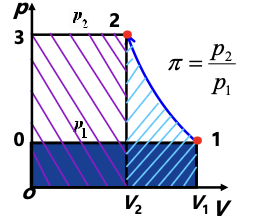
\includegraphics[width=.8\linewidth]{figures/8单级活塞式压气机.png}
\end{minipage}

\pt{压力比}：$\pi=\frac{p_2}{p_1}$

\pt{压气机耗功}：$W_C=\int_1^2V\,\mathrm{d}p=-W_t$，单位质量 $w_C=\int_1^2v\,\mathrm{d}p=-w_t$。生产量常用单位时间生产气体的标准立方米表示，不同于进、排气状态体积。

\noindent
\begin{minipage}
    [t]{0.48\linewidth}
    \vspace{0pt}
    \raggedright
    \pt{理论耗功}：$-w_t=\Delta h-q$，$w_C$ 取决于初终态及过程特征。理想气体：
    \begin{itemize}
        \item \pt{绝热压缩} $q=0$：$w_{C,s}=h_{2s}-h_1=\frac{\kappa}{\kappa-1}R_{\mathrm{g}}T_1\left(\pi^\frac{\kappa-1}{\kappa}-1\right)$。
        \item \pt{等温压缩} $\Delta h=0$：$w_{C,T}=R_{\mathrm{g}}T_1\ln\pi$。
        \item \pt{多变压缩}：$w_{C,n}=\frac{n}{n-1}p_1v_1\left(\pi^\frac{n-1}{n}-1\right)$。
    \end{itemize}

    \pt{压缩过程比较}：$w_{C,s}>w_{C,n}>w_{C,T}$，$T_{2s}>T_{2n}>T_{2T}$，$v_{2s}>v_{2n}>v_{2T}$；\\通常为多变压缩 $1<n<\kappa$，\\$n\uparrow$ 时 $w_{C,n},T_{2n},v_{2n}$ 均增大；\\理想压缩为\pt{等温压缩}。
\end{minipage}
\hfill
\begin{minipage}
    [t]{0.48\linewidth}
    \vspace{0pt}
    \centering
    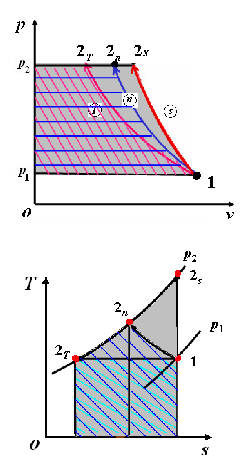
\includegraphics[width=.8\linewidth]{figures/8三种压缩.png}
\end{minipage}

\divider

\noindent
\begin{minipage}
    [t]{0.48\linewidth}
    \vspace{0pt}
    \raggedright
    \pt{余隙容积 $V_c$}：产生于进、排气结构布置、制造装配公差、部件热膨胀等。
    工作过程：
    \begin{itemize}
        \item $1$-$2$ 压缩
        \item $2$-$3$ 排气
        \item $3$-$4$ 余隙气体膨胀
        \item $4$-$1$ 吸气
    \end{itemize}
\end{minipage}
\hfill
\begin{minipage}
    [t]{0.48\linewidth}
    \vspace{0pt}
    \centering
    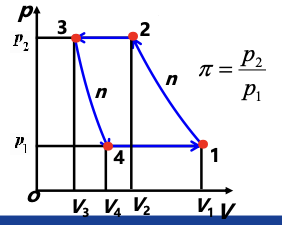
\includegraphics[width=.8\linewidth]{figures/8带余隙容积的压缩.png}
\end{minipage}

\pt{余隙相关容积}：$V_c=V_3$，气缸工作容积 $V_h=V_1-V_3$，\\有效吸气容积 $V_{\mathrm{es}}=V_1-V_4$，余隙容积比 $\sigma=\frac{V_c}{V_h}$。\\\pt{每周期生产量} $m_{\mathrm{pr}}=m_1\frac{V_1-V_4}{V_1}$。

\noindent
\begin{minipage}
    [t]{0.58\linewidth}
    \vspace{0pt}
    \raggedright
    \pt{容积效率}：$\eta_V=\frac{V_{\mathrm{es}}}{V_h}=\frac{V_1-V_4}{V_1-V_3}=1-\frac{V_3}{V_1-V_3}\left(\frac{V_4}{V_3}-1\right)=1-\sigma\left(\pi^{1/n}-1\right)$。
    \begin{itemize}
        \item $V_c,V_h$ 定时：$\pi\uparrow\Rightarrow\eta_V\downarrow,m_p\downarrow$。
        \item $\pi$ 定时：$V_c\uparrow\Rightarrow V_{\mathrm{es}}\downarrow,\eta_V\downarrow,m_p\downarrow$。
    \end{itemize}
\end{minipage}
\hfill
\begin{minipage}
    [t]{0.38\linewidth}
    \vspace{0pt}
    \centering
    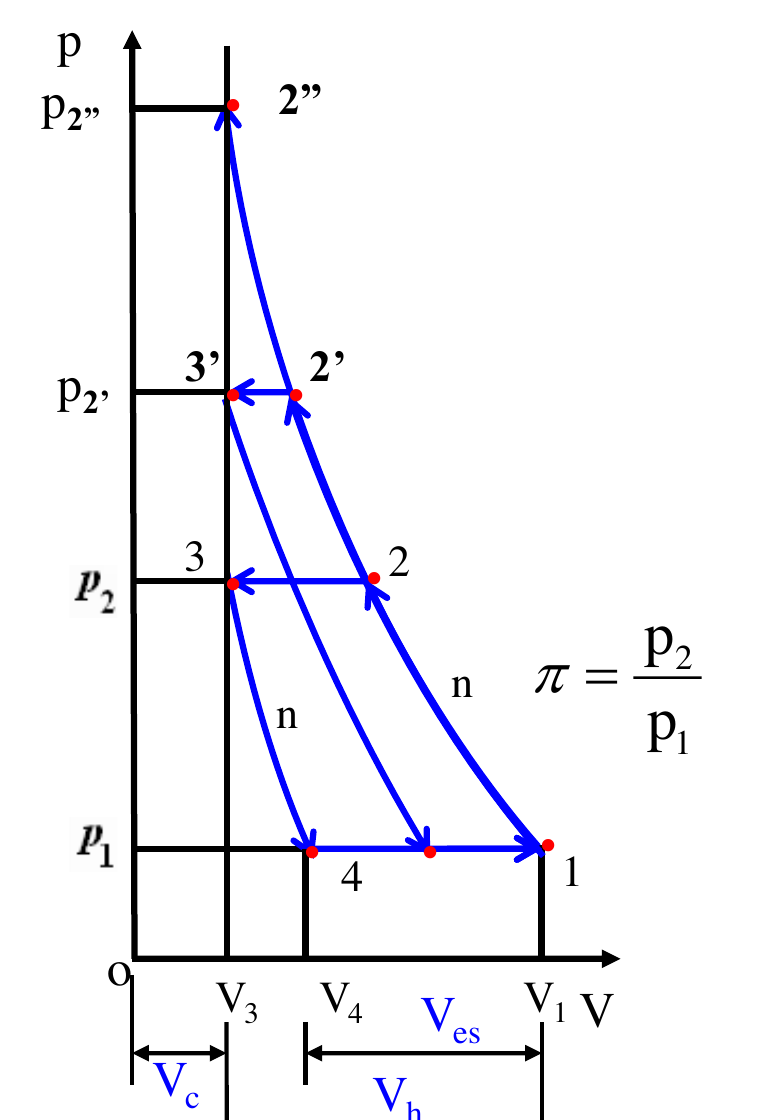
\includegraphics[width=.8\linewidth]{figures/8余隙容积效率影响.png}
\end{minipage}

\pt{余隙对理论耗功}：$W_C=W_{t,1-2}-W_{t,3-4}=\frac{n}{n-1}p_1(V_1-V_4)\left(\pi^{(n-1)/n}-1\right)$；因 $V_{\mathrm{es}}=m_{\mathrm{pr}}v_1$，故 $w_C=\frac{W_C}{m_{\mathrm{pr}}}=\frac{n}{n-1}v_1p_1\left(\pi^{(n-1)/n}-1\right)$。余隙使生产量下降、实际耗功增大，但对生产 $1\,\mathrm{kg}$ 气体的理论耗功无影响，故称有害容积。

\divider


\pt{叶轮式压气机}：包括轴流式、离心式；转速高，连续吸排气，运转平稳，排气量大，无余隙影响，但每级压比不高。因排量大、转速高、难冷却，常按\pt{绝热压缩}分析。

\noindent
\begin{minipage}
    [t]{0.56\linewidth}
    \vspace{0pt}
    \raggedright
    \pt{叶轮式绝热分析}：理论耗功 $w_{C,s}=h_{2s}-h_1$，实际耗功 $w'_C=h_{2'}-h_1$，实际多耗功 $\Delta w_C=h_{2'}-h_{2s}$。绝热内效率
    $\eta_{C,s}=\frac{w_{C,s}}{w'_C}=\frac{h_{2s}-h_1}{h_{2'}-h_1}$；理想气体时 $\eta_{C,s}=\frac{T_{2s}-T_1}{T_{2'}-T_1}$，$T_{2'}=T_1+\frac{T_{2s}-T_1}{\eta_{C,s}}=T_1+\frac{w_{\mathrm{c}}'}{c_\mathrm{p}}$。
\end{minipage}
\hfill
\begin{minipage}
    [t]{0.40\linewidth}
    \vspace{0pt}
    \centering
    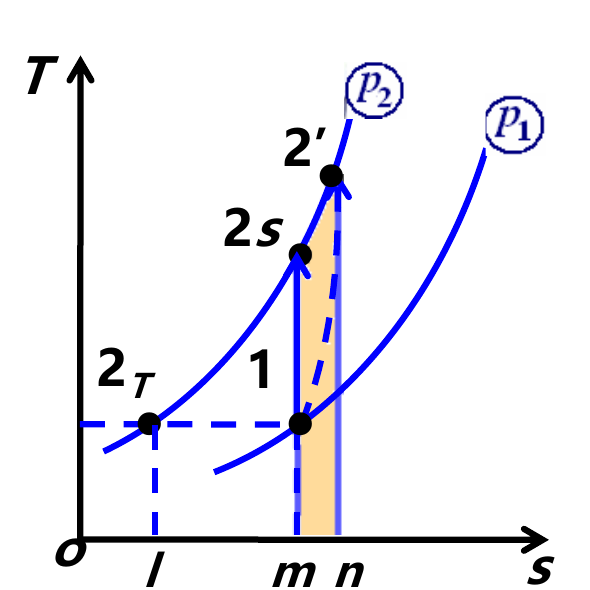
\includegraphics[width=.8\linewidth]{figures/8叶轮式Ts图.png}
\end{minipage}

\newpage

\pt{多级压缩与级间冷却}：高压气体压缩时 $p\uparrow$ 使 $T\uparrow$、$\eta_V\downarrow$，常受 $T_2\leq T_{2,\max}$、$\eta_V\geq\eta_{V,\min}$ 限制，故采用分级压缩、级间冷却。

%\noindent
%\begin{minipage}
%    [t]{0.52\linewidth}
%    \vspace{0pt}
%    \raggedright
%    \pt{多级压缩与级间冷却}：高压气体压缩时 $p\uparrow$ 使 $T\uparrow$、%$\eta_V\downarrow$，常受 $T_2\leq T_{2,\max}$、$\eta_V\geq\eta_%{V,\min}$ 限制，故采用分级压缩、级间冷却。
%\end{minipage}
%\hfill
%\begin{minipage}
%    [t]{0.44\linewidth}
%    \vspace{0pt}
%    \centering
%    \includegraphics[width=.8\linewidth]{figures/8多级压缩装置.png}
%\end{minipage}

\noindent
\begin{minipage}
    [t]{0.56\linewidth}
    \vspace{0pt}
    \raggedright
    \pt{二级压缩耗功}：每生产 $1\,\mathrm{kg}$ 气体，$w_C=w_{C,L}+w_{C,H}$。若中冷后 $T_3=T_1$，令 $a=\frac{n-1}{n}$，$\pi_L=\frac{p_a}{p_1}$，$\pi_H=\frac{p_2}{p_a}$，则 $w_C=\frac{nR_{\mathrm{g}}T_1}{n-1}(\pi_L^a+\pi_H^a-2)$。
\end{minipage}
\hfill
\begin{minipage}
    [t]{0.40\linewidth}
    \vspace{0pt}
    \centering
    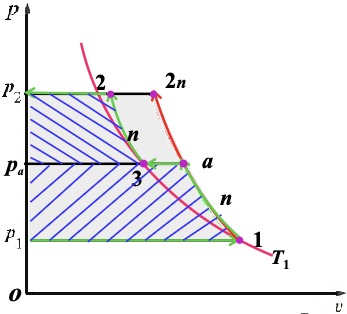
\includegraphics[width=.8\linewidth]{figures/8二级压缩耗功图.png}
\end{minipage}

\pt{最佳中间压力}：令 $\frac{\partial w_C}{\partial p_a}=0$，得 $p_a=\sqrt{p_1p_2}$，即 $\pi_L=\frac{p_a}{p_1}=\frac{p_2}{p_a}=\pi_H$，此时 $w_C=w_{C,\min}$。推广到 $m$ 级：$\pi_1=\pi_2=\cdots=\pi_m=\left(\frac{p_2}{p_1}\right)^{1/m}$。

\pt{等压比分级优点}：各级耗功相等 $w_{C,i}=\frac{n}{n-1}R_{\mathrm{g}}T_1\left(\pi_i^{(n-1)/n}-1\right)$，$w_C=mw_{C,i}$；各缸终温相同 $T_i=T_1\pi_i^{(n-1)/n}$；各级缸散热 $q_i=\frac{n-\kappa}{n-1}c_{\mathrm{V}}\Delta T$、中冷器散热 $q_{\mathrm{中},i}=c_p\Delta T$ 相等；各缸按比例缩小，利于曲轴平衡、润滑可靠和提高整机 $\eta_V$。

\noindent
\begin{minipage}
    [t]{0.56\linewidth}
    \vspace{0pt}
    \raggedright
    \pt{级数影响}：$m\uparrow$ 时趋近等温压缩；但体积庞大、系统复杂、可靠性下降，工程常用 $2$--$4$ 级。\\\pt{定温效率} $\eta_{C,T}=\frac{w_{C,T}}{w_C}$。\\\pt{真空泵}实质也是压气机：出口压力为环境压力，进气压力不断降低。
\end{minipage}
\hfill
\begin{minipage}
    [t]{0.40\linewidth}
    \vspace{0pt}
    \centering
    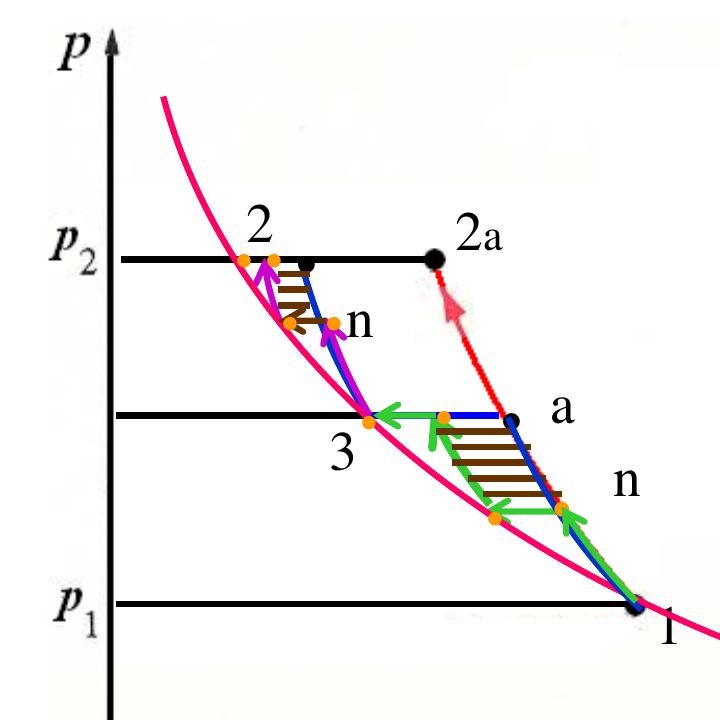
\includegraphics[width=.8\linewidth]{figures/8四级压缩趋等温.png}
\end{minipage}

\divider

